\section{Activity Forecasting}

\begin{frame}
	\frametitle{Future Directions}
	\framesubtitle{Activity forecasting}
	
	\vspace{0.4cm}
	
	Kitani \emph{et al.} proposed a novel method for activity forecasting
	by combining:
	
	\begin{itemize}
		\item Semantic scene understanding
		\vspace{0.05cm}
		\item Inverse Reinforcement Learning
	\end{itemize}
	
	\begin{center}
		\begin{tikzpicture}
			\node at (0,0) [draw=white,ultra thick,inner sep=0pt]
			{
				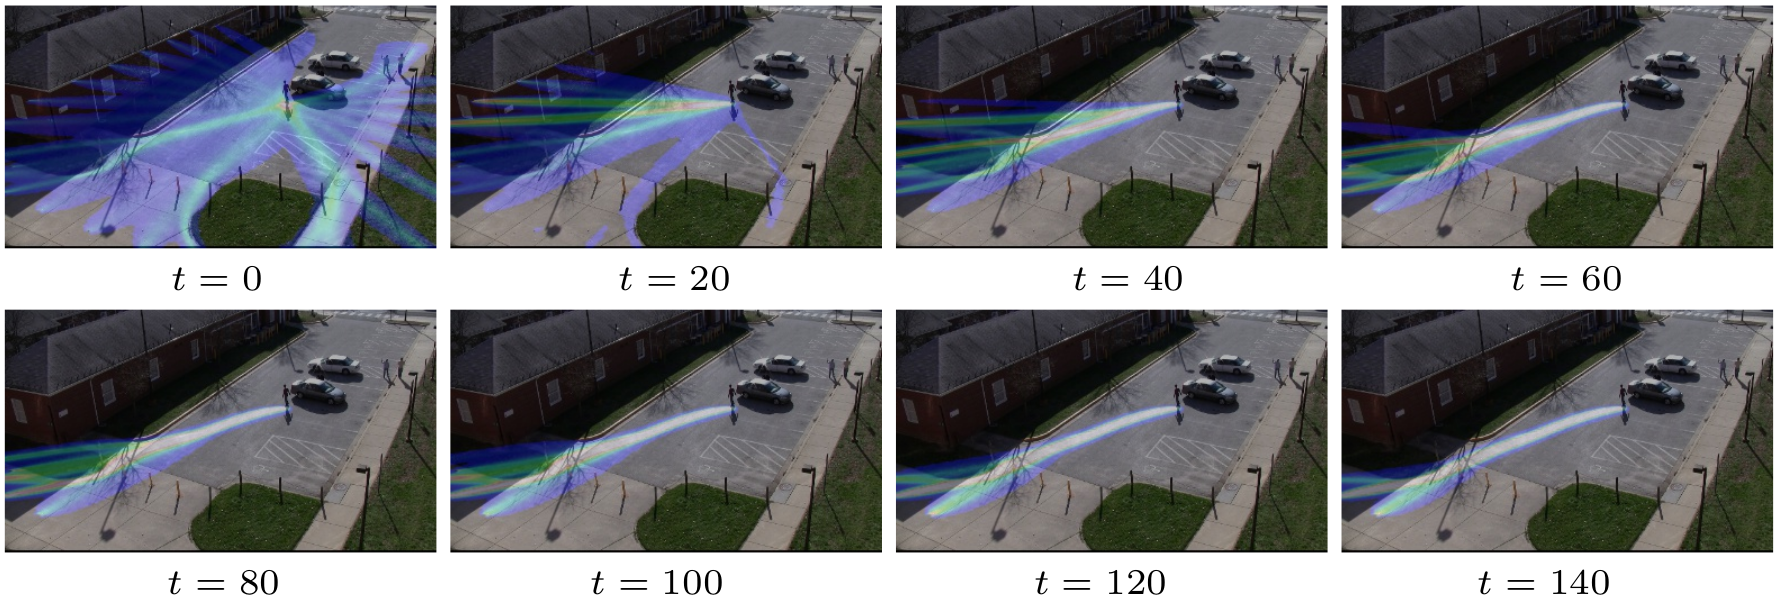
\includegraphics[scale=0.19]{Figures/ActivityForecasting.png}
			};
		\end{tikzpicture}
	\end{center}
\end{frame}

\begin{frame}
	\frametitle{Activity Forecasting}
	
	\vspace{0.35cm}
	
	\begin{block}{Idea}
		Performing activity forecasting resolving an \textbf{Inverse Reinforcement
		Learning} problem \textbf{without} needing a labeled environment, by combining:
		
		\begin{itemize}
			\item object trajectories provided by \emph{PTracking}
			\item representation of the environment following the \emph{grid world} schema
				  defined by Russell \emph{et al.}
		\end{itemize}
	\end{block}
	
	\begin{center}
		\begin{tikzpicture}
			\node at (0,0) [draw=white,ultra thick,inner sep=0pt]
			{
				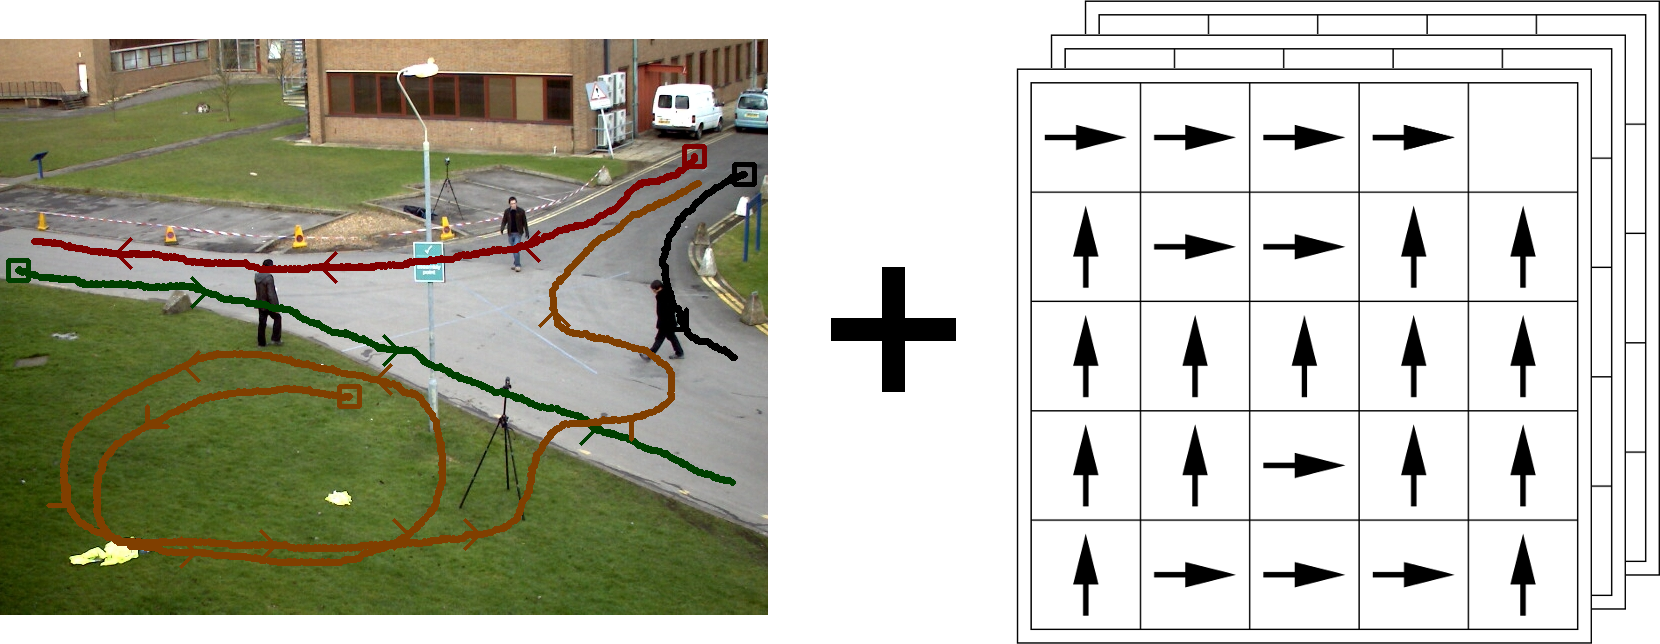
\includegraphics[height=3.2cm]{Figures/IRL}
			};
		\end{tikzpicture}
	\end{center}
\end{frame}

\begin{frame}
	\frametitle{Activity Forecasting}
	\framesubtitle{IRL problem}
	
	\large
	
	\begin{eqnarray*}
		maximize \sum_{i=1}^N min_{a \in \{a_1, \ldots, a_k \}} \Big \{ [ \mathbf{P}_{a_*}(i) - \mathbf{P}_a(i) ] ( \mathbf{I} - \gamma \mathbf{P}_{a_*})^{-1} \mathbf{R} \Big \} - \lambda \| \mathbf{R} \|_1 \\ \\
		s.t. \;\;\; (\mathbf{P}_{a_*} - \mathbf{P}_a)(\mathbf{I} - \gamma \mathbf{P}_{a_*})^{-1} \mathbf{R} \succeq 0 \;\;\;\;\;\;\;\; \forall a \in A \; \backslash \; a_* \;\;\;\;\;\;\;\;\;\;\;\;\;\;\;\;\;\;\;\; \\
		| \mathbf{R}_i | \leq R_{max} \;\;\;\;\;\;\;\;\;\;\;\;\;\;\;\;\;\;\;\;\;\;\;\;\;\;\;\;\;\;\;\;\;\;\;\;\; i \in \{ 1, \ldots, N \} \;\;\;\;\;\;\;\;\;\;\;\;\,\,
	\end{eqnarray*}
	
	\vspace{0.2cm}
	
	where
	
	\begin{itemize}
		\item $ \mathbf{R} $ is the \textbf{reward} vector
		\item $ \mathbf{P}_a $ is the \textbf{state transition probabilities} for action
			  $ a $
		\item $ \mathbf{P}_a(i) $ denotes the $ i $-th row of $ \mathbf{P}_a $
		\item $ \gamma $ is the \textbf{discount factor}
		\item $ \lambda $ is a \textbf{penalty factor}
	\end{itemize}
\end{frame}

\begin{frame}
	\frametitle{Activity Forecasting}
	\framesubtitle{Reward function}
	
	\begin{center}
		\begin{tikzpicture}
			\node at (0,0) [draw=white,ultra thick,inner sep=0pt]
			{
				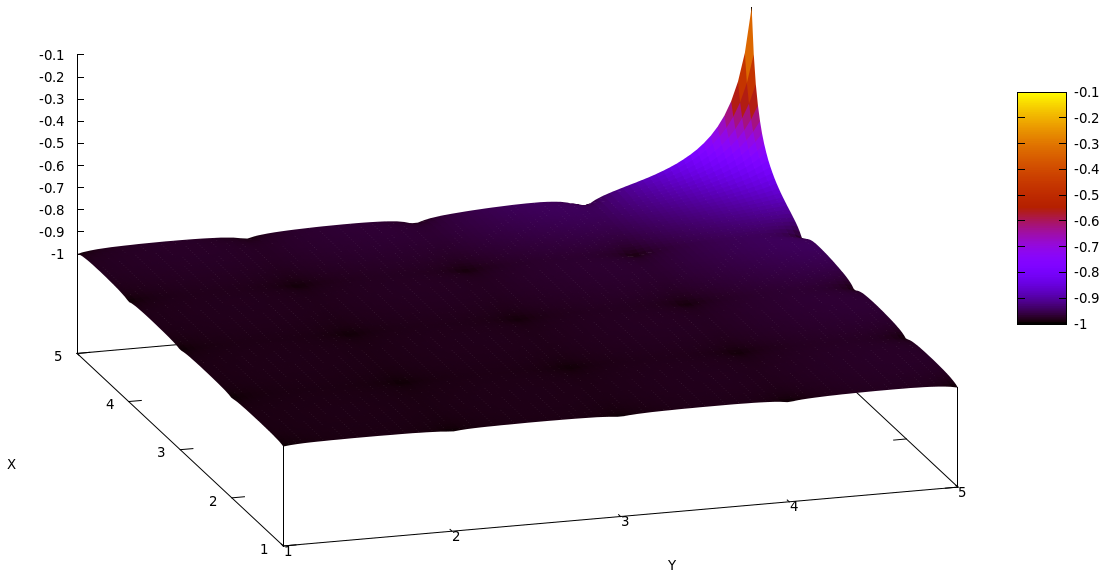
\includegraphics[width=\linewidth]{Figures/Reward}
			};
		\end{tikzpicture}
	\end{center}
\end{frame}
